%% ============================================================
%%  SOLUCIÓN — Ejercicio 3.2: Insertar una figura
%%  Clase 1 — Después de diapositiva "Insertar figuras"
%%  NOTA: Requiere una imagen llamada 'mi_figura.png' en la misma carpeta
%%  Compilar: F5 (pdflatex)
%% ============================================================

\documentclass[12pt, a4paper]{article}
\usepackage[utf8]{inputenc}
\usepackage[T1]{fontenc}
\usepackage[spanish]{babel}
\usepackage{graphicx}

\title{Visualización de datos de salarios}
\author{Tu Nombre}
\date{\today}

\begin{document}
\maketitle

\section{Distribución de salarios}

Como se observa en la Figura \ref{fig:salarios}, la distribución del salario 
presenta sesgo positivo. Esto significa que hay pocos valores muy altos que 
jalan la media hacia la derecha.

% NOTA: Si no tienes la imagen, comentá las líneas siguientes para que el documento compile
% Si sí la tienes, descomenta las líneas y asegurate de que 'mi_figura.png' esté en la misma carpeta

\begin{figure}[htbp]
  \centering
  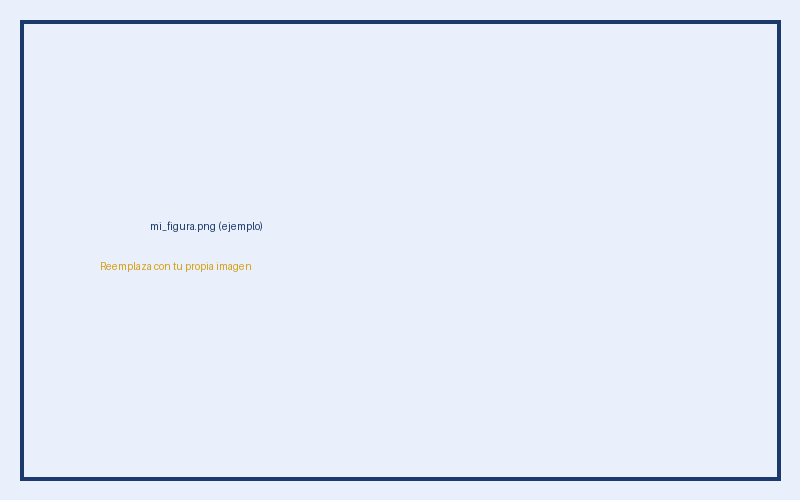
\includegraphics[width=0.65\textwidth]{mi_figura}
  \caption{Distribución del salario mensual (en logaritmos)}
  \label{fig:salarios}
\end{figure}

\section*{Parámetro [htbp]}

El parámetro \texttt{[htbp]} indica a \LaTeX{} dónde preferentemente colocar 
la figura:
\begin{itemize}
  \item \texttt{h} = ``here'' (aquí, donde la escribo)
  \item \texttt{t} = ``top'' (arriba de la página)
  \item \texttt{b} = ``bottom'' (abajo de la página)
  \item \texttt{p} = ``page'' (en una página solo de figuras)
\end{itemize}

\LaTeX{} intenta respetar este orden de preferencias, pero si la figura no 
cabe, la mueve.

\section*{Opciones de ancho}

Algunos ejemplos de cómo controlar el tamaño:
\begin{itemize}
  \item \texttt{width=0.65\textbackslash textwidth} — 65\% del ancho de la página
  \item \texttt{width=10cm} — exactamente 10 centímetros
  \item \texttt{height=8cm} — altura exacta
  \item \texttt{scale=0.8} — 80\% del tamaño original de la imagen
\end{itemize}

\end{document}
